\documentclass{article}
\usepackage[left=2cm,right=2cm,top=2cm,bottom=2cm]{geometry}
\usepackage[utf8]{inputenc}
\usepackage[german]{babel}
\usepackage{amsmath}
\usepackage{dsfont}
\usepackage[export]{adjustbox}
\usepackage{amsthm}
\usepackage{color}
\usepackage{amsfonts}
\usepackage{amssymb}
\usepackage{wasysym}
\usepackage{makeidx}
\usepackage{graphicx}
\usepackage[colorlinks=true,urlcolor=blue,linkcolor=blue]{hyperref}
\usepackage{ziffer}
\usepackage{minted}
\usepackage{xcolor}
\usepackage{framed}
\usepackage{mdframed}
\usepackage{subfiles}
\usemintedstyle{emacs}

\definecolor{purp}{HTML}{9A72AC}
\definecolor{re}{HTML}{FC6255}
\definecolor{gre}{HTML}{83C167}
\definecolor{blu}{HTML}{58C4DD}
\definecolor{shadecolor}{rgb}{0.85,0.85,0.85}
\definecolor{bg}{rgb}{0.95,0.95,0.95}
\setlength{\parindent}{0em} 

\BeforeBeginEnvironment{minted}{\begin{mdframed}[linewidth =2 ,backgroundcolor=bg , linecolor=black, linewidth=0.5]}
\AfterEndEnvironment{minted}{\end{mdframed}}

\newtheorem{defi}{Definition}
\BeforeBeginEnvironment{defi}{\begin{mdframed}[linewidth =2 ,backgroundcolor=bg , linecolor=black, linewidth=0.5]}
\AfterEndEnvironment{defi}{\end{mdframed}}

\newcommand{\bsp}{\textbf{Beispiel}:}
%\newcommand{\task}{\textbf{Aufgabe}:}

\newcommand{\bol}[1]{\textbf{#1}}
\newcommand{\q}[1]{\glqq #1\grqq}
\newcommand{\DODO}[1]{\textbf{\textcolor{red}{DODO:}} #1 \\ \begin{center}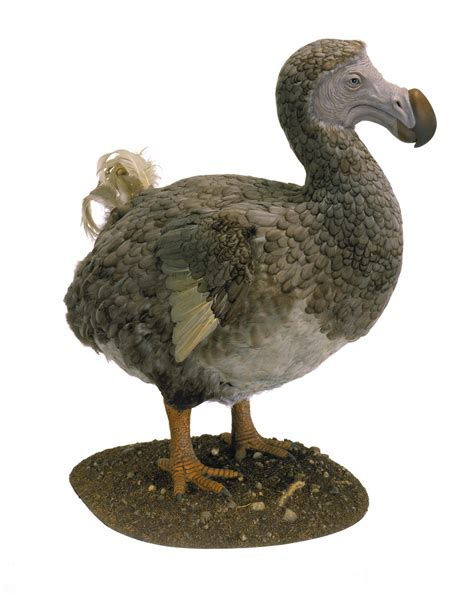
\includegraphics[scale=0.2]{../../media/dodo.jpg} \end{center}}

\newenvironment{task}[1]{
    \begin{shaded*}
    \textbf{Aufgabe #1}:
}{
    \end{shaded*}
}

\begin{document}

\subsection{Die Tiefensuche}

Anders als bei Bäumen oder Listen gibt es bei Graphen keinen \q{besonderen} Knoten, der als Einstiegspunkt für Algorithmen dient, bzw. die Struktur vorgibt. Es gibt verschiedene Arten einen Graphen zu traversieren, dabei wird ausgehend von einem (zufällig) ausgewählten Startknoten der gesamte Graph durchlaufen. Zunächst beschäftigen wir uns mit der sogenannten \textbf{Tiefensuche}. Wie der Name bereits sagt, fokussiert sich diese Art zu suchen darauf, zunächst einen möglichst \q{tiefen} oder \q{langen} Weg innerhalb des Graphen zu finden. Im Gegensatz dazu arbeitet sich die \textbf{Breitensuche} \q{ebenenweise} durch den Graphen. (siehe nächstes Kapitel) \\
Einige Anwendugsbereiche der Tiefensuche sind: 
\begin{itemize}
    \item \textbf{Entkommen aus einem Labyrinth:} Wir starten an einem Ort des Labyrinths und versuchen durch intelligentes Ausprobieren aller Lösungsmöglichkeiten einen Pfad aus dem Labyrinth zu finden. 
    \item \textbf{Routing:} Die Tiefensuche ist eine Möglichkeit einen Weg durch ein Netzwerk zu finden. 
    \item \textbf{Machine Learning:} Graphen spielen auch im maschinellen Lernen eine große Rolle, auch hier kann die Tiefensuche gewinnbringend eingesetzt werden.
\end{itemize}

Das grundlegende Vorgehen hat mehrere Schritte:
\begin{enumerate}
    \item[1] Der Algorithmus wird auf einem beliebigen Knoten gestartet.
    \item[2] Der aktuelle Knoten wird als besucht markiert. 
    \item[3] Es wird geprüft, ob es noch unbesuchte Nachbarknoten gibt. 
    \item[3.1] Falls ja: Rekursion! Die Methode wird auf einem unbesuchten Nachbarknoten aufgerufen
    \item[3.2] Falls nein: Die Methode ist für den aktuellen Knoten beendet und es wird zurück zu 2 gesprungen.  
\end{enumerate}
Der Algorithmus endet dann, wenn keine der Methodenaufrufe mehr übrig ist. Dadurch, dass wir die Methode auf einem weiteren Knoten aufrufen, anstatt zuerst alle Nachbarknoten abzuarbeiten, erhält die Tiefensuche die Eigenschaft möglichst weit \q{in die Tiefe} zu gehen. Erst wenn wir keine weitere Möglichkeit mehr finden gehen wir \q{zurück nach oben}.
\begin{center}
    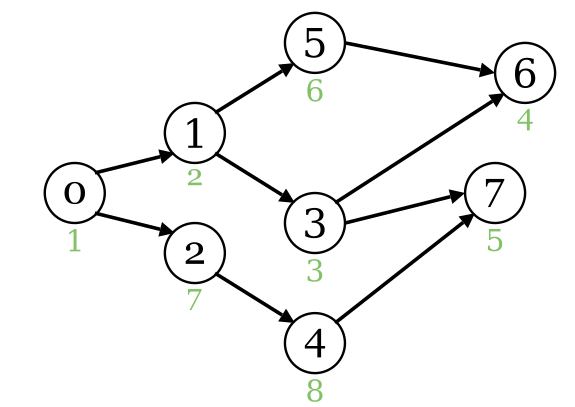
\includegraphics[scale=0.35]{../media/depth_search.png}
\end{center}
\href{https://youtu.be/nM9hBCUMXMA}{\textbf{Zugehöriges Video}}\\
Beginnen wir beim Knoten $0$, so haben wir zwei Möglichkeiten zu starten, entweder den Knoten $1$ oder $2$. Im Zweifel wird in dieser Implementierung der Knoten mit der niedrigeren Nummer gewählt, d.h. die Tiefensuche wird auf $1$ aufgerufen. Das Entscheidende ist jetzt, dass der nächste Schritt von $1$ aus geführt wird, nicht von $2$ (der Methodenaufruf auf $2$ erfolgt erst nach der vollständigen Abarbeitung des Methodenaufrufs auf $1$). $1$ ruft deswegen als Nächstes die Methode auf $3$ auf, dieser Knoten danach auf $6$. Jetzt sind wir an einem \q{toten Ende} angekommen, es gibt keine weiteren unbesuchten Nachbarn und wir gehen \q{eine Ebene zurück}. \\
In diesem Fall ist das Knoten $3$. Hier sind wir aber noch nicht fertig, da es einen weiteren unbesuchten Nachbarn von $3$ gibt, nämlich die $7$. Wieder sind wir in einer Sackgasse und schließen die Methoden für $7$ und $3$ ab und kehren zur $1$ zurück. Nachdem jetzt die $5$ abgearbeitet ist, wird endlich auch der Methodenaufruf der $1$ beendet und in einem letzten Schritt $2$ und dann $4$ besucht (die $7$ ist bereits markiert und wir nicht nochmal besucht, auch wenn sie am Ende dieses Pfades steht!). Insgesamt ergibt sich der folgende Durchlauf:
\begin{center}
    $0 \rightarrow 1 \rightarrow 3 \rightarrow 6 \rightarrow 7 \rightarrow 5 \rightarrow  2 \rightarrow 4$
\end{center}
\textbf{Zur Implementierung:} \\
Das Wesentliche Element, das uns in unserer derzeitigen Implementierung des Graphen noch fehlt, ist eine Möglichkeit zu speichern, ob ein Knoten bereits besucht wurde. Hier gibt es viele Implementierungsmöglichkeiten, z.B.:
\begin{itemize}
    \item Jeder Knoten hat ein entsprechendes Attribut
    \item Es gibt ein Boolean-Array, das genausoviele Einträge hat wie es Knoten gibt und als Attribut des Graphen gespeichert ist.
    \item Das angesprochene Array könnte auch bei Methodenaufruf erzeugt werden und eine Referenz darauf \q{mitgegeben werden}
\end{itemize}
Im Folgenden wird die zweite Methode verwendet, d.h. wir ergänzen in unserem Graphen ein entsprechendes Attribut, das im Konstruktur initialisiert wird.
\begin{minted}{java}
public class Graph {

    private double[][] matrix;
    private Node[] nodes;
    private boolean[] visited;

    public Graph(int nodeNumber) {
        nodes = new Node[nodeNumber];
        for(int i = 0; i < nodeNumber; i++) {
            nodes[i] = new Node(i);
        }
        matrix = new double[nodeNumber][nodeNumber];
        visited = new boolean[nodeNumber];
    }
}
\end{minted}
Die eigentliche Suche ist zweigeteilt, zunächst müssen wir den Startknoten spezifizieren und dann die Rekursion starten - man könnte hier von einer Helfermethode sprechen, hier initialisieren wir auch das \q{Besucht}-Array.
\begin{minted}{java}
public void depthSearchStart(int nodeNumber) {
    //Das Array muss jedes Mal neu initialisiert werden, damit alle Einträge false sind.
    //Alternativ könnte man am Ende der Rekursion das Array zurücksetzen. 
    visited = new boolean[nodes.length];
    depthSearch(nodeNumber, "");
}
\end{minted}
Die eigentliche Rekursion geschieht dann in der \textit{depthSearch} Methode (im Folgenden mit Kommentaren):

\begin{minted}{java}
private void depthSearch(int nodeNumber, String indent){
    //Der aktuelle Knoten wird abgearbeitet
    visited[nodeNumber] = true; 
    //Zum Testen: Ausgabe einer Einrückung (wird bei jedem Aufruf erweitert)
    // und anschließend der Nummer des besuchten Knotens
    System.out.println(indent + nodeNumber);
    for(int i = 0; i < nodes.length; i++) {
        //Für jeden Knoten werden alle anderen Knoten angesehen, falls es eine Kante gibt
        // und der Knoten nicht besucht ist, wird die Rekursion dort forgesetzt.
        if(matrix[nodeNumber][i] != 0 && !visited[i]) {
            depthSearch(i, indent + " ");
        }
    }
}
\end{minted}
Dadurch, dass Java Methodenaufrufe auf den internen Stack legt, wird hier der Weg \q{in die Tiefe} sichergestellt, denn bevor in unserer Wiederholung der zweite potentielle Nachbar angesehen wird, wird die gesamte Rekursion auf dem ersten Nachbarn ausgeführt, d.h. so tief wie möglich in dessen Abschnitt des Graphen durch die entsprechenden rekursiven Methodenaufrufe(siehe auch Veranschaulichungsvideo!). 
\newpage
\subsection{Breitensuche}

Die grundlegende Idee der Breitensuche ist der Tiefensuche sehr ähnlich, der Graph wird entlang der Kanten langsam abgesucht. Im Gegensatz zur Tiefensuche, werden aber alle \q{zuerst} gefundenen Knoten abgearbeitet. D.h. anstatt sich auf den Stapel der Methodenaufrufe zu verlassen, muss eine Warteschlange zur Verwaltung verwendet werden. Das grundlegende Vorgehen sieht wie folgt aus:
\begin{enumerate}
    \item Der Algorithmus wird auf einem beliebigen Knoten gestartet.
    \item Der aktuelle Knoten wird als besucht markiert.
    \item Wenn es noch unbesuchte Nachbarknoten gibt, werden diese zur Warteschlange hinzugefügt. 
    \item Der erste Knoten in der Warteschlange wird entfernt und auf ihm rekursiv die Breitensuche aufgerufen.
\end{enumerate}

Wir betrachten denselben Graphen wie zuvor: 
\begin{center}
    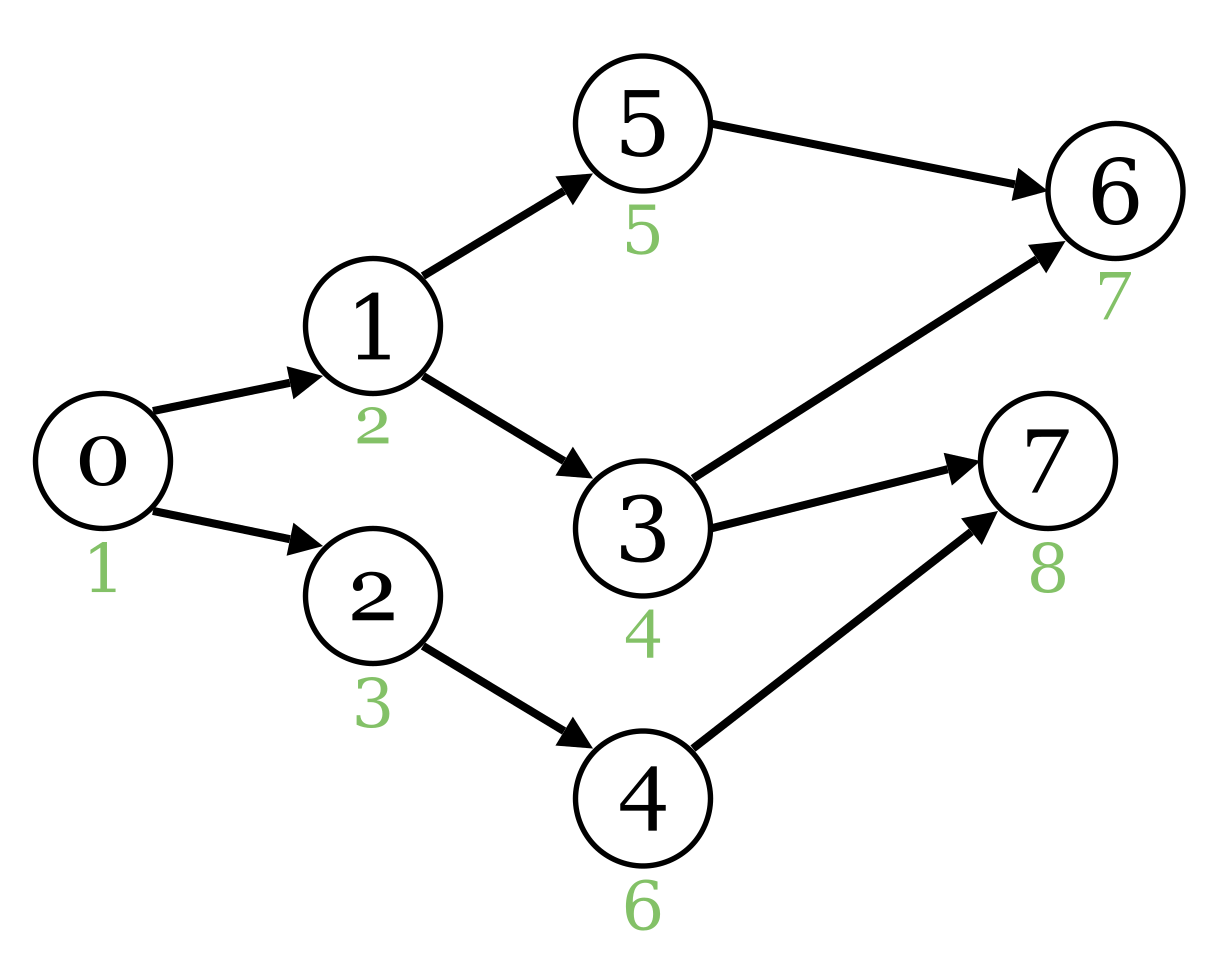
\includegraphics[scale=0.15]{../media/broad_search.png}
\end{center}
\href{https://youtu.be/pgRzRGii0F4}{\textbf{Zugehöriges Video}}\\
Wir beginnen wieder beim Knoten $0$, es werden die Knoten $1$ und $2$ (wieder in der Reihenfolge der Nummerierung) in die Warteschlange eingefügt. Danach wird das erste Element aus der Warteschlange entfernt, in diesem Fall die $1$. Von hier aus wird die $3$ und die $5$ in die Warteschlange aufgenommen. \\
Im Gegensatz zur Tiefensuche geht es jetzt aber bei Knoten $2$ weiter, da dieser vorne in der Warteschlange steht und 4 wird in die Warteschlange aufgenommen. Im weiteren Verlauf wird nun $3$ aus der Warteschlange entfernt und daraufhin $6$ und $7$ aufgenommen. Insgesamt ergibt sich folgender Durchlauf:
\begin{center}
    $0 \rightarrow 1 \rightarrow 2 \rightarrow 3 \rightarrow 5 \rightarrow 4 \rightarrow 6 \rightarrow 7$
\end{center}
\textbf{Zur Implementierung:} \\
Wir orientieren uns an der bereits implementierten Tiefensuche. Neben dem bereits erläuterten \q{visited}-Array wird eine Warteschlange benutzt. An dieser Stelle könnte die Anfang des Jahres erarbeitete Warteschlangen-Implementierung verwendet werden, in der Praxis würde man eher auf vorgefertigte Java-Implementierungen zurückgreifen, z.B. auf eine LinkedList (diese implementiert in Java das Queue-Interface, ist also als Warteschlange geeignet). Die LinkedList befindet sich im \q{util}-Package und muss importiert werden (Verwendet man die LinkedList im Code wird VsCode automatisch den entsprechenden Import schreiben)
\begin{minted}{java}
 public class Graph {

    private double[][] matrix;
    private Node[] nodes;
    private boolean[] visited;
    private LinkedList<Integer> queue;

    // ...
}
\end{minted}
Da wir nur die Nummern der Knoten in die Warteschlange stellen müssen, da wir über diese Nummern ohnehin die entsprechenden Knoten im Knoten-Array ansprechen, genügt es eine LinkedList von Integern zu erstellen (die Klammern $<>$ legen fest, welchen \q{Inhalt} bzw. welche Daten in der LinkedList gespeichert werden sollen). \\
Wir beginnen wieder mit der Start-Methode:
\begin{minted}{java}
public void broadSearchStart(int nodeNumber) {
    visited = new boolean[nodes.length];
    //Es muss jedes Mal eine neue Warteschlange erzeugt werden!
    queue = new LinkedList<Integer>();
    broadSearch(nodeNumber);
}
\end{minted}
Die eigentliche Breitensuche wird wieder in der \textit{broadSearch}-Methode ausgeführt:
\begin{minted}{java}
public void broadSearch(int nodeNumber) {
    //Der aktuelle Knoten wird als besucht markiert
    visited[nodeNumber] = true;
    //Zum Testen: Ausgabe des aktuellen Knoten und einer kurzen Notiz
    System.out.println(nodeNumber + " visited!");
    for(int i = 0; i < nodes.length; i++) {
        //Für jeden Knoten wird überprüft, ob er ein Nachbarknoten ist und
        //ob er noch nicht besucht ist
        if(matrix[nodeNumber][i] != 0 && !visited[i]) {
            //Falls beides der Fall ist wird der Knoten zur Warteschlange hinzugefügt
            queue.addLast(i);
        }
    }
    //Es wird überprüft, ob die Warteschlange leer ist, falls nein
    //wird das vorderste Element entfernt und die Breitensuche auf ihm aufgerufen
    //Erinnerung: in der Warteschlange stehen direkt die Integer, die den
    //Positionen der Knoten entsprechen.
    if(!queue.isEmpty()) broadSearch(queue.pop());
}
\end{minted}
In dieser Implementierung werden auch Knoten an die Warteschlange angehängt, die bereits in der Warteschlange sind. Der mehrfache Aufruf der Methode auf einem Knoten schadet zwar dem Algorithmus nicht, ist aber auch nicht vollkommen effizient. Die Prüfung, ob ein Element bereits in der Warteschlange ist bedeutet einen relativ großen Aufwand, da über die gesamte Warteschlange iteriert werden muss, im Allgemeinen ist die Warteschlange zwar deutlich kleiner als die Anzahl der Knoten des Graphen, kann aber trotzdem relativ lang sein. \\
Die einfachste Variante das Problem zu lösen ist, den Knoten bereits als besucht zu markieren, wenn er in die Warteschlange hinzugefügt wird, da er ab diesem Zeitpunkt auf jeden Fall besucht wird. Die veränderte Methode sieht dann so aus:
\begin{minted}{java}
public void broadSearchStart(int nodeNumber) {
    visited = new boolean[nodes.length];
    //Es muss jedes Mal eine neue Warteschlange erzeugt werden!
    queue = new LinkedList<Integer>();
    //Da nicht mehr am Anfang der Methode hinzugefügt wird muss hier der Anfangsknoten
    // extra gesetzt werden
    visited[nodeNumber] = true;
    broadSearch(nodeNumber);
}

public void broadSearch(int nodeNumber) {
    //Zum Testen: Ausgabe des aktuellen Knoten und einer kurzen Notiz
    System.out.println(nodeNumber + " visited!");
    for(int i = 0; i < nodes.length; i++) {
        //Für jeden Knoten wird überprüft, ob er ein Nachbarknoten ist und
        //ob er noch nicht besucht ist
        if(matrix[nodeNumber][i] != 0 && !visited[i]) {
            //Falls beides der Fall ist wird der Knoten zur Warteschlange hinzugefügt
            queue.addLast(i);
            //Der hinzugefügte Knoten wird bereits als besucht markiert
            visited[nodeNumber] = true;
        }
    }
    //Es wird überprüft, ob die Warteschlange leer ist, falls nein
    //wird das vorderste Element entfernt und die Breitensuche auf ihm aufgerufen
    if(!queue.isEmpty()) broadSearch(queue.pop());
}
\end{minted}

Möchte man die Knoten nicht \q{zu früh} markieren gibt es auch noch eine andere Variante, die Verwendung eines \textbf{HashSets}. In dieser Datenstruktur kann die Frage, ob ein Element in ihr vorhanden ist, im durchschnittlichen Fall in $\mathcal{O}(1)$ beantwortet werden. Wir können damit verwalten, welche Knoten bereits in der Warteschlange sind, bzw. waren. \\
Im Folgenden eine erweiterte Form der der Breitensuche mit einem \textbf{HashSet}:
\begin{minted}{java}
public class Graph {

    private boolean[] visited;
    private LinkedList<Integer> queue;
    //Die Menge wird definiert
    private HashSet<Integer> indicesInQueue;
    private double[][] matrix;
    private Node[] nodes;

    //...
    
    public void broadSearchStart(int nodeNumber) {
        visited = new boolean[nodes.length];
        queue = new LinkedList<Integer>();
        //Wie die Warteschlange muss die Menge initialisiert werden, es genügen wieder 
        //Integer als Positionen der Knoten
        indicesInQueue = new HashSet<Integer>();
        //Der erste Knoten wird aufgenommen.
        indicesInQueue.add(nodeNumber);
        broadSearch(nodeNumber);
    }

    public void broadSearch(int nodeNumber) {
        visited[nodeNumber] = true;
        for(int i = 0; i < nodes.length; i++) {
            //Zusätzlich zu zuvor wird nun überprüft, ob i bereits in der Warteschlange war
            if(matrix[nodeNumber][i] != 0 && !visited[i] && !indicesInQueue.contains(i)) {
                queue.addLast(i);
                //Falls nein wird i der Menge hinzugefügt. 
                indicesInQueue.add(i);
            }
        }
        if(!queue.isEmpty()) broadSearch(queue.pop());
    }
}
\end{minted}


\newpage
\subsection{Anwendungsaufgaben}

\begin{task}{1}
Schreiben Sie eine Methode, die testet, ob ausgehend von einem Startknoten ein bestimmter Zielknoten erreichbar ist. 
\end{task}

\begin{task}{2}
    Schreiben Sie eine Methode, die testet, ob ein ungerichteter Graph zusammenhängend ist.
\end{task}

\begin{task}{3}
Schreiben Sie eine Methode, die testet, ob ein gerichteter Graph stark zusammenhängend ist. 
\end{task}

\begin{task}{4}
Schreiben Sie eine Methode, die testet, ob es in einem gerichteten Graphen mindestens einen Knoten gibt, von dem aus alle anderen erreichbar sind.
\end{task}

\begin{task}{5}
Schreiben Sie eine Methode, die testet, ob ein gerichteter Graph schwach zusammenhängend ist. 
\end{task}

Die Lösungen finden sich wie immer auf der nächsten Seite.

\newpage 

Eine Methode, die testet, ob ein Pfad zwischen zwei Knoten vorhanden ist kann einfach direkt auf die Tiefensuche zurückgreifen. Wenn danach im visited-Array an der Stelle des Endknotens ein \textbf{true} steht, wird dies entsprechend zurückgegeben. \\
\begin{minted}{java}
public boolean testPath(int start, int end) {
    depthSearchStart(start);
    return visited[end];
}
\end{minted}
Man könnte natürlich auch die Tiefensuche so modifizieren, dass sie abbricht, sobald end gefunden wurde. Das würde die Laufzeit ggf. noch optimieren. \\
Um einen ungerichteten Graphen auf Zusammenhang zu testen muss einfach nur die Tiefensuche ausgeführt werden und danach das visited-Array untersucht werden. Steht an irgendeiner Stelle \textbf{false}, so ist der Graph nicht zusammenhängend.
\begin{minted}{java}
public boolean testConnection() {
    depthSearchStart(0);
    for(int j = 0; j < visited.length; j++) {
        if(!visited[j]) return false;
    }
return true;
} 
\end{minted}

Ist der Graph dagegen gerichtet, so muss für den starken Zusammenhang die Tiefensuche von jedem Knoten aus gestartet werden, da zwar von einem Knoten aus alle erreichbar sein können, durch die Richtung der Kanten ein \q{umgekehrter} Weg aber nicht zwingend notwendig ist. Dennoch erfordert dieses Problem nur eine kleine Modifikation:
\begin{minted}{java}
public boolean testConnectionStrong(){
    for(int i = 0; i < nodes.length; i++) {
        depthSearchStart(i);
        for(int j = 0; j < visited.length; j++) {
            if(!visited[j]) return false;
        }
    }
    return true;
}    
\end{minted}

Für Aufgabe 4 muss der obige Code nur leicht modfiziert werden, es wird nicht mehr automatisch false zurückgegeben, sondern nur dieser Durchlauf abgebrochen, wenn ein \textbf{false} im visited-Array gefunden wird:
\begin{minted}{java}
public boolean testConnectionOneNode(){
    for(int i = 0; i < nodes.length; i++) {
        depthSearchStart(i);
        int counter = 0;
        for(int j = 0; j < visited.length; j++) {
            counter++;
            if(!visited[j]) break;
        }
        if(counter == visited.length) {
            return true;
        }
    }
    return false;
}
\end{minted}
Für den schwachen Zusammenhang muss der Graph in einen ungerichteten Graphen umgewandelt werden. Damit wir den Graphen nicht überschreiben und seine Informationen verlieren, basteln wir einen zweiten Graphen aus den vorhandenen Informationen. Anschließend können wir einfach die testConnection()-Methode für ungerichtete Graphen verwenden.
\begin{minted}{java}
public boolean testWeakConnection() {
    int n = matrix.length;
    double[][] newMatrix = new double[n][n];
    Node[] newNodeList  = new Node[n];
    for (int i = 0; i < n; i++) {
        nodes[i] = new Node(i);
    }
    for(int i = 0; i < n; i++) {
        for(int j = i + 1; j < n; j++) {
            if(matrix[i][j] != 0) {
                newMatrix[i][j] = 1;
                newMatrix[j][i] = 1;
            }
        }
    }
    Graph g2 = new Graph(newMatrix, newNodeList);
    return g2.testConnection();
}
\end{minted}

